\documentclass[12pt]{article}

\usepackage{sbc-template}
\usepackage[T1]{fontenc}
\usepackage{graphicx,url}
\usepackage{array}
\usepackage{color}
\usepackage{listings}
\usepackage{fancyhdr}
\usepackage[T1]{fontenc}
\usepackage{epsfig}
\usepackage{rotating}
\usepackage{setspace}

\usepackage[square,
            authoryear,
            sort&compress,]{natbib}
\let\cite=\citep

\usepackage[brazilian]{babel}
\usepackage[utf8]{inputenc}

     
\sloppy

\title{ProLine-RM - Tool to Manager Crosscutting Framework Families}

\author{Rafael S. Durelli\inst{1}, Valter V. de Camargo\inst{2}}


\address{Computer  Systems Department University of S\~{a}o Paulo\\
  S\~{a}o Carlos, SP, Brazil.
\nextinstitute
  Computing Departament\\ Federal University of S\~{a}o Carlos (UFSCAR)\\
  S\~{a}o Carlos, SP, Brazil.
  \email{rdurelli@icmc.usp.br\inst{1}, valter@dc.ufscar.br\inst{2}}
}

\begin{document} 

\maketitle

\begin{abstract}
  Abstract will be here.
\end{abstract}


\section{Introduction}


\section{Motivation} \label{sec:motivation}

In the literature, it is possible find out a lot of researches related to CFF (COLOCAR REF). However, to the best of our knowledge, there is neither an approach nor a tool that shares, manages and provides full cycle of reuse of the CFF. Moreover, it is important a tool that supplies a graphical way to allow the engineer examines previously if the features available in one CFF fulfill the application requirements. %Moreover, it is important that there is way to allow the engineer verify whether the variability/features available in the CFF meet the application requirements that must be developed.  

%Afterwards, the features have been examined and chosen by the engineer it is likewise important provides a way to download only the artifacts that have been chosen.    

%Thus, the CFF can be used during a development process easier and can be provided major computer support to facilitate such as task.     

%It is important that there is a way to examine whether the variability / features available in the family of FTs meet the application requirements that must be developed. In order for families of FTs to be properly used during a development process, and a major computer support to facilitate this task.

In order to overcome such limitations we have put forward a plug-in named Product Line-Repository Manager (ProLine-RM) which implements complete cycle of reuse of the CFF. Using this plug-in the CFF can be reused in a controlled way during the reuse to increase the quality of the developed applications. Furthermore, any manipulation in the CFF can be made through the intermediary of models, so we intend to raise the level of abstraction in which the engineer works.


%Thus, the objective of this paper is describes this plug-in. 

%Embora v�rios autores j� tenham trabalhado com FTs (Couto et al., 2005; Hanenberg et al., 2004; Huang et al., 2004; Shah e Hill, 2004; Constantinides e Elrad, 2001; Pinto et al., 2002; Rashid e Chitchyan, 2003; Soares et al., 2006; Vanhaute et al., 2001; Huang et al., 2004; Mortensen e Ghosh, 2006a; Mortensen e Ghosh, 2006b; Soares, 2004), n�o � encontrado na literatura o projeto de um reposit�rio de FTs e t�cnicas para busca de um determinado FT que atenda aos requisitos de uma aplica��o. � importante que exista uma forma de averiguar se as variabilidades/caracter�sticas dispon�veis na fam�lia de FTs atendem aos requisitos da aplica��o que deve ser desenvolvida. Para que fam�lias de FTs sejam adequadamente usadas durante um processo de desenvolvimento, � importante um apoio computacional que facilite essa tarefa.


\section{ProLine-RM} \label{sec:proline}

In this section, we present the ProLine-RM tool, which is useful for providing full cycle of reuse of the CFF. The ProLine-RM has been developed upon the Eclipse Plugin License~\footnote{www.eclipse.org} (EPL). The use of the tool is twofold, the Domain Engineering (DE) phase where all artifacts are developed and upload to a repository, and the Application Engineering (AE) phase, where the reuse is done effectively. In order to illustrate the ProLine-RM in the DE phase and its functionalities we describe all activities necessaries to devise a ``persistence'' CFF. Similarly, to illustrate how the ProLine-RM assists the engineer in the AE phase we have developed an application that use the ``persistence'' CFF. These phases are described in the next two sections, respectively.

\subsection{Domain Engineering}  

Figure~\ref{fig:proline} depicts a screenshot of ProLine-RM. In this figure the DE phase is exhibits by letter ``A'' to ``C''. 
%In order to illustrated the useful of the ProLine-RM and its functionalities we describe all activities necessaries to devise a ``persistence'' CFF. 
In the first step the domain related to ``persistence'' has been studied. 
The outcome of such study were the identification of both the common features and its variants of the domain. 

After identifying the all features of the CFF the next activity is the development of the CFF effectively (see Figure~\ref{fig:proline}(A)). For the purpose of accomplishing this activity we have used the approach described by~\citet{deCamargo:2008:PDC:1363686.1363863}, its aims is to assists and makes easier the develop of the CFF by using aspect oriented paradigm~\cite{Kiczales97aspect-orientedprogramming}. 

Afterwards, the feature model depicting all features related to the domain has to be modeled. 
Aiming to make easier the development of feature models, ProLine-RM provides a graphical way to assists the engineer devise them. 
Figure~\ref{figu:progile}(B) shows the feature model that we have developed. 
As can be seen, there are two mandatory features. 
The first one, called ``Persistence'' aims to introduce a set of persistence operations into application persistence classes (e.g., store, remove, update, perform queries). 
The second feature, named ``Connection'' is related to the database connection concern and identifies points in the application code where the connection must be opened and closed. 
This feature has variabilities, as for example Data Base Management System (e.g., MySQL, SyBase, Native and Interbase).
There are two optional features as well. The former is called ``Caching'', which is responsible to deal with high-performance to get datas of the databases.
The second, named ``Pooling'' is represented a set of database connections maintained by the databases.

After developing all artifacts, them have to be uploaded in a repository in order to be reused during the AE phase.
Prior to uploading these artifacts, informations (e.g., Named of CFF, Author(s) and Description) associated with the ``persistence'' CFF has to be filled in. Figure~\ref{fig:proline}(C) shows an example wherein the CFF is being uploaded.

\subsection{Application Engineering}

As stated previously, in the AE phase is wherein the reuse is started effectively.

\begin{figure}[!h]
\centering
  % Requires \usepackage{graphicx}
 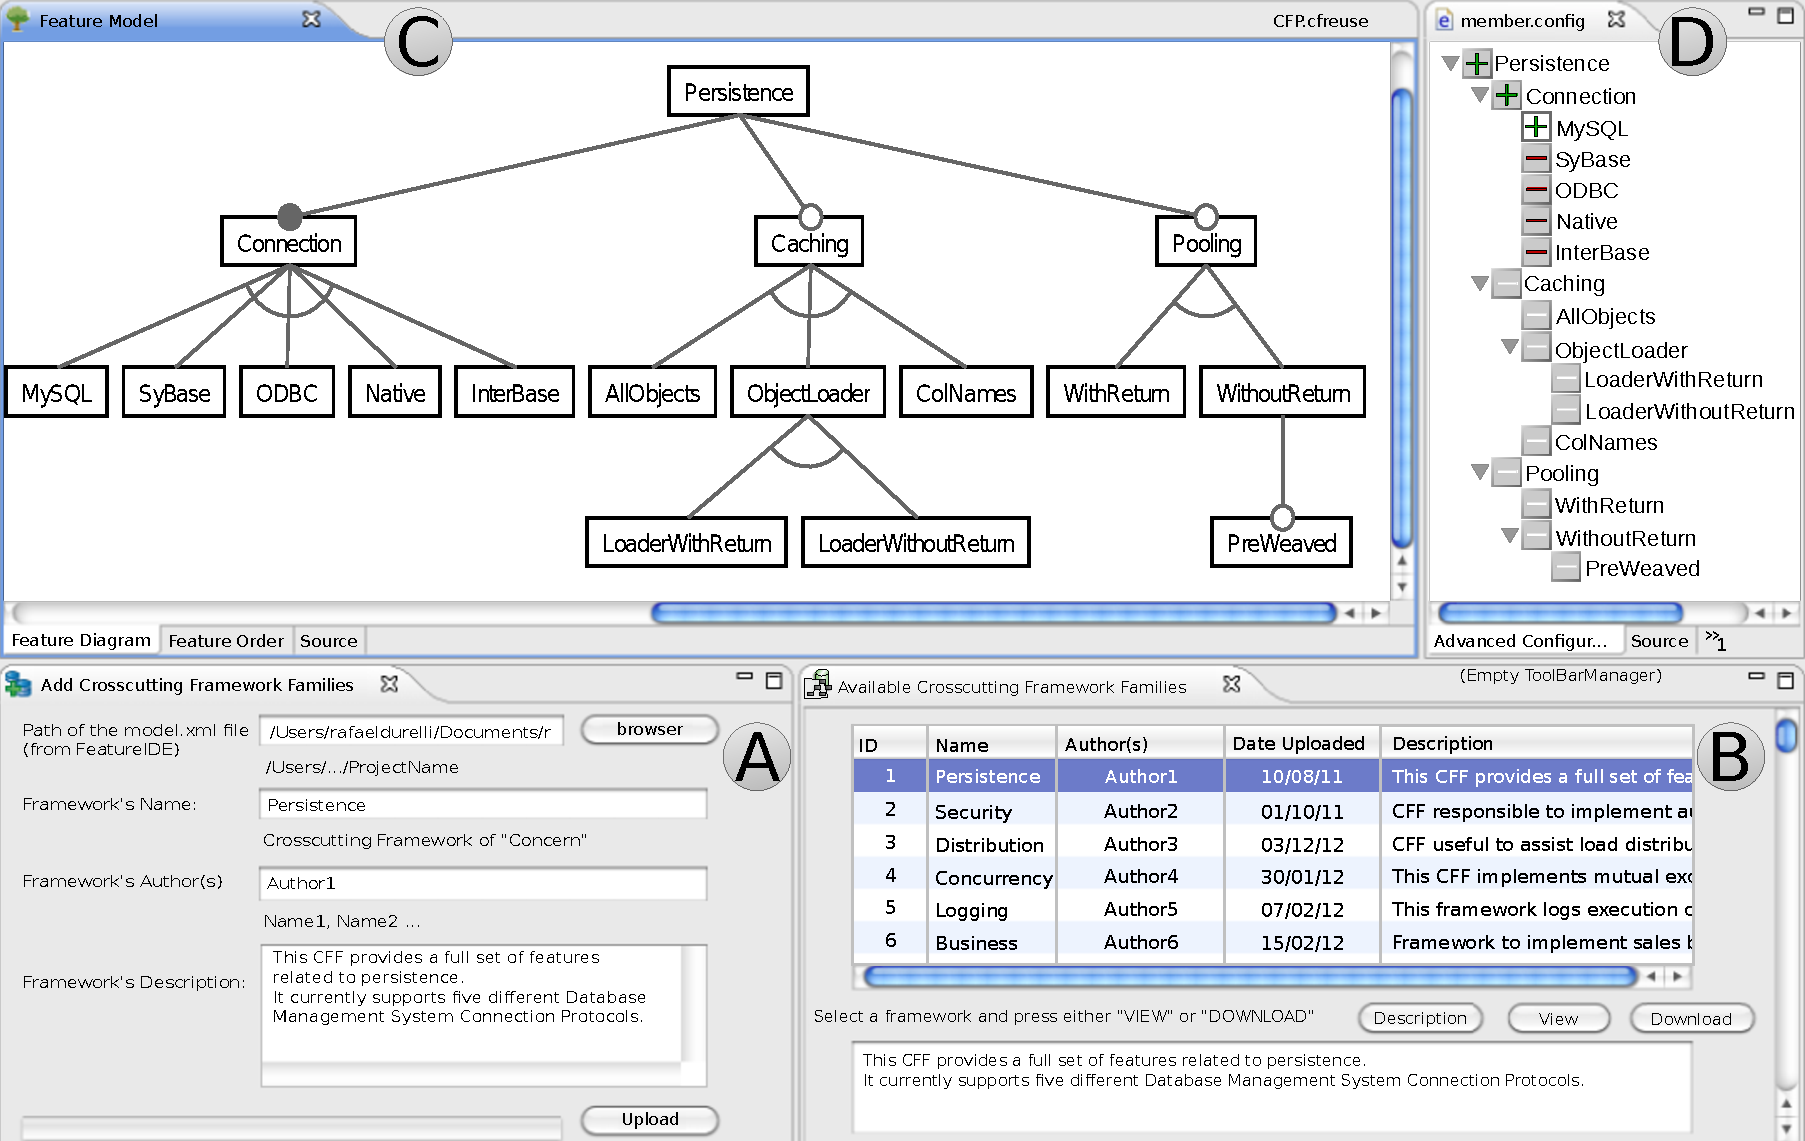
\includegraphics[scale=0.065]{figuras/PROLINERM}
\caption{Screenshot of ProLine-RM}
\label{fig:proline}
\end{figure}    

     
%To the best of our knowledge, there is no an approach that shares, managements, provides full cycle of reuse of the CFF and even supplies a way to examine previously if the features available in one CFF fulfill the application requirements. In order to overcome these absence we put forward an approach and a tool named Proline-RM acronym for Product Line-Repository Manager, which aims to increase the level of manager and accelerate the instantiation of members belonging to a given CFF. The use of the approach is twofold, the Domain Engineering (DE) where all artifacts are developed and upload to a remote server, and the Application Engineering (AE), where the reuse is done effectively. 

\subsection{ProLine-RM Architecture}\label{sec:architecture}

\section{Related Work}\label{sec:related}

\section{Concluding Remarks}\label{sec:conclusion}

\section{Acknowledgements}


\bibliographystyle{apalike}
\bibliography{sbc-template}

\end{document}
